\documentclass{memoir}

%\usepackage{fancyhdr}
\usepackage{xcolor}
\usepackage{hyperref}
\usepackage{graphicx}
\usepackage{enumitem}
\usepackage{verbatim}
\usepackage{framed}

\setlength{\parindent}{0pt}
\nonzeroparskip


\graphicspath{{../figures/}}
\hypersetup{
  colorlinks,
  linkcolor={red!50!black},
  citecolor={blue!50!black},
  urlcolor={blue!80!black}
}
\urlstyle{same}
\setlength{\headheight}{15.2pt}
\pagestyle{simple}
%\fancyhf{}
%\lfoot[$\the\numexpr\value{page}$]{} %-1 to take into account title page.
%\rfoot[]{$\the\numexpr\value{page}$}

\begin{document}

\chapter{Introduction}
\label{chap:introduction}

\section{Disclaimers}
\label{sec:disclaimers}

It is very important that the user realises that I wrote this program, in the first place, for personal use, and that I only make it available for free in case other people may find it helpful in their work. However, you will use the program at your own risk. I do \textbf{not} take any responsibility for problems that you run into when using the program. That being said, I am always open to receiving comments, positive or negative, about problems that may occur, bugs you encounter, features you would like to be included, and so on. If you do indeed run into problems as a result of using this program, I am willing to help you think of a solution. You can find my contact details in chapter \ref{chap:contactdetails} of this manual.

The user should also realise that I am \textbf{not} a professional programmer. With some help from the Internet, I taught myself how to code to keep my mind occupied during some of the lonely evening hours I spent in an campus apartment somewhere in Shenyang. I never had any formal training in writing code, and I probably make a lot of ugly mistakes, write inefficient code, and overlook simple solutions for the various problems I face while writing code. While I always try to improve my coding skills, this requires a lot of time, energy, and verbal abuse of my computers\footnote{If you happen to be someone with more experience at writing code, feel free to go to my Github page (see chapter\ref{chap:contactdetails}) to inspect the source code of this program, and if you have the time and patience, please offer me suggestions on how to improve my skills.}. This means that I will not always have the time, energy and/or the skills required to fix certain bugs, add new features, and etcetera.

I also do \textbf{not} have a team of beta-testers to help me test the program. You are basically it. Congratulations! If I had T-shirts, I would ship you one to give you some recognition, but unfortunately I have no budget for that. The program is still fairly simple in structure, and I tried to get rid of most bugs by doing my own testing. However, the program is already complex enough for me to overlook things, so there is a good possibility to several annoying bugs remain. The only way to find these, sadly, is to encounter them while using the program. Fortunately for you, if there is one thing that I really hate, it is having bugs in my programs. If you do encounter a bug, please contact me (see chapter \ref{chap:contactdetails}) ASAP, and I (or we) will try to figure out what is wrong, so that I can fix it.



\chapter{Preparations}
\label{chap:preparations}

\section{Data sets}
\label{sec:datasets}


\subsection{Other notes}
\label{sec:othernotesdatasets}

The program is not able to read csv-files that have so-called newline symbols (\textbackslash n) or carriage return symbols (\textbackslash r) in their text cells. The reason for this is that the program uses a relatively simple csv-file parser, which will think that a new line of data will start after encountering one of these symbols (each line of data in a csv-file will end with a newline symbol by default). The program is typically able to recognise when an 'illegal' newline is encountered, and it will throw an error (see figure \ref{fig:importerror}). Solving the error is left to the user. The problem can be solved by removing all newline symbols and carriage return symbols from the csv-file with the dataset. These symbols are not visible in programs like Excel or LibreOffice Calc, and in both programs you will need to use special search and replace options to get rid of the unwanted symbols. I advise you to Google for ``Find and replace regular expressions with [your spreadsheet program]''. 

\chapter{Using the program}
\label{chap:usingtheprogram}

\section{Loading a new dataset}
\label{sec:loadingnewdataset}

Importing the new data into the program works as follows. You first need to select the csv-file containing your data. For this you will click the \textbf{Select File} button (see figure \ref{fig:importoptions}), which will open a file dialog that you can use to navigate to, and select the file.

Once a file has been selected, you will need to select the delimiter symbol that is used in the csv-file to distinguish between different columns of the data table. For this, you can use the dropdown menu that reads \textbf{-Select delimiter-} by default. Four different symbols are allowed as delimiter, which are the comma (,), the semicolon (;), the colon (:), and the vertical bar (\textbar). Make sure that the delimiter that you select matches the one used in the file.

Once you have selected a delimiter, you can import the data, using the \textbf{Import data} button. Once you click this button, the program will attempt to read data from selected file and, if successful, enable all other options of the program, allowing you to start coding.   

\begin{figure}[h!]
  \centering
  \caption{Options to import data.}
  \includegraphics[width=100mm]{Screenshot_0.pdf}
  \label{fig:importoptions}
\end{figure}

\subsection{Problems when importing data}
\label{sec:importerrors}

If you (1) selected a valid csv-file, (2) selected the correct delimiter for this file, and (3) structured your data set using instructions offered in section \ref{sec:datasets}, you should encounter no problems when importing the data. If something goes wrong when importing data, then the problem will usually lie with one of these three points.

One possibility is that you have not selected a valid csv-file. I have encountered a few people that have tried to create csv-files from (for example) xls-files by simply changing the file extension. Doing this will not actually create a valid csv-file that can be read by the program. The correct way for creating csv-files is to use the \textbf{Save as} option in your spreadsheet editor, and select to save the file with the \textbf{*.csv} extension.

If you selected the wrong delimiter, the program will usually import the data, but it will fail to distinguish between different columns of the data set, and possibly assume that the entire dataset only contains one column. This should be obvious from the texts displayed by the program. In this case, simply import the data again, using the correct delimiter. 

If you see the error message displayed in figure \ref{fig:importerror}, this means that some cells of your data set probably contain newline symbols and/or carriage return symbols that need to be removed before importing data (see section \ref{sec:othernotesdatasets}).

\begin{figure}[h!]
  \centering
  \caption{Data import error report.}
  \includegraphics[width=40mm]{Screenshot_1.pdf}
  \label{fig:importerror}
\end{figure}

If you are certain that you made no mistakes in one of these points, and you still encounter problems when importing your data set, then you may have encountered a bug in the program that needs to be fixed. In that case, please get in touch with me (see chapter \ref{chap:contactdetails}).

\section{Saving and loading data}
\label{sec:savingloadingdata}

Coding a data set typically will take a long time, which is why the program allows you to save your progress, and to load the saved session at another moment. Saving data can be done by clicking the \textbf{Save current session} button (see figure \ref{fig:saveload}). A file dialog will appear, asking you to select a location to store the file, as well as a name for the file. The files will always be saved with the ``.sav'' extension.

If you want to load a previously stored session, click the \textbf{Load previous session} button (see figure \ref{fig:saveload}). A file dialog will appear, allowing you to navigate to, and select the file that you wish to load. 

\begin{figure}[h!]
  \centering
  \caption{Saving and loading files.}
  \includegraphics[width=100mm]{Screenshot_2.pdf}
  \label{fig:saveload}
\end{figure}

\section{Importing existing codes}
\label{sec:importingcodes}

Coding data is typically an iterative process, and it is possible that, during the coding process, the user makes changes to the data set being coded, for example, by adding new rows of data, by adding new columns of data, or by changing the contents of data cells. The program therefore allows the user to import existing codes from an old version of a given data set into a new version of the same data set. 

\begin{figure}[h!]
  \centering
  \caption{Importing codes.}
  \includegraphics[width=100mm]{Screenshot_3.pdf}
  \label{fig:importcodesfig}
\end{figure}

The procedure for importing codes involves the following steps:
\begin{enumerate}
\item{The user should first make sure that the codes assigned to the \textbf{old version} of the data set are stored, by using the \textbf{Save session option} (see section \ref{sec:savingloadingdata}). At a later step, we will import the codes from this save file. For this example, we refer to this files as \textbf{Saved\textunderscore Codes.sav}.}
\item{After saving the codes assigned to the \textbf{old version} of the data set, we can import the \textbf{new version} of the data set, using the procedure described in section \ref{sec:loadingnewdataset}. Thus, the steps taken here are the same as when you would start coding a completely new data set.}
\item{After the \textbf{new version} of the dataset has been loaded, you should click the \textbf{Import codes} button (see figure \ref{fig:importcodesfig}). You will first be shown a warning dialog, just to make sure that you can double check what you are doing. If you select \textbf{Ok} in the warning dialog, you will be shown a file dialog. Use this dialog to find the file with your saved codes (\textbf{Saved\textunderscore Codes.sav} in this example). Select and open this file.}
\item{A new dialog will appear, the specific contents of which will depend on the contents of your data sets. An example is shown in figure \ref{fig:importcodesfig}, but yours will probably look different. The dialog will show the columns that the old version of your data set and the new version of your data set have in common. Here, you need to select those columns that the program can use to match entries in the \textbf{old version} of the data set with entries in the \textbf{new version} of the data set. The program will look at the data in the selected columns of both files. If it finds a row of data in the \textbf{new version} of the data set and a row of data in the \textbf{old version} of the data set that have the exact same contents in the selected columns, then the program will decide that these rows of data are the same. The program will then ensure that all the codes that are somehow associated with the row of data in the \textbf{old version} of the data set, are also associated with the corresponding row of data in the \textbf{new version} of the data set. For this to work correctly, the rows of data in both data sets need to be unique. For example, if you select only one column, which has the same contents in multiple rows in one or both of the data sets, then the program will not be able to decide which codes are associated with which row of data. \textbf{In this case the codes will probably be assigned to the new data set erroneously, without warning!\footnote{In a later version of the program I will attempt to prevent this from happening altogether.} It is therefore very important that you always select a combination of columns that allows the program to identify each row of data individually.} Usually, it should be enough to select the column that indicates the timing of the incident, and the column that describes what happened in that incident, because having two incidents with the exact same timing, and the exact same contents (description) would probably never make sense, because they would describe the same (inter)action, making one of them redundant. See figure \ref{fig:importingcodesdiagram} for a schematic overview that may help to understand the process.}
\item{You also have the option to have the program mark any new entries in the \textbf{new version} of the data set. This means that, while checking the columns you have selected, the program will also remember any rows of data in the \textbf{new version} of the data set that it could not match to any rows of data in the \textbf{old version} of the data set. These entries will be marked (see \ref{sec:markingincidents}), so that you can easily find them while coding the data.}
\item{If you happened to have changed data in one of the rows of the data set, that is, the row was already present in the \textbf{old version} of the data set, but you changed some of the contents of that row of data in the \textbf{new version} of the data set (in one of the selected columns), that row of data will be treated as new entry, and any codes assigned to that entry will be lost.}
\item{The program should now return to the main screen, and any attribute codes and relationship codes that were present in the save file that you loaded should now also be available in the current session. Moreover, any incidents that already had codes assigned to them in that save file should now also have those codes assigned to them in the current session.}
\end{enumerate}

\begin{figure}[h!]
  \centering
  \caption{Schematic overview of matching of data set entries.}
  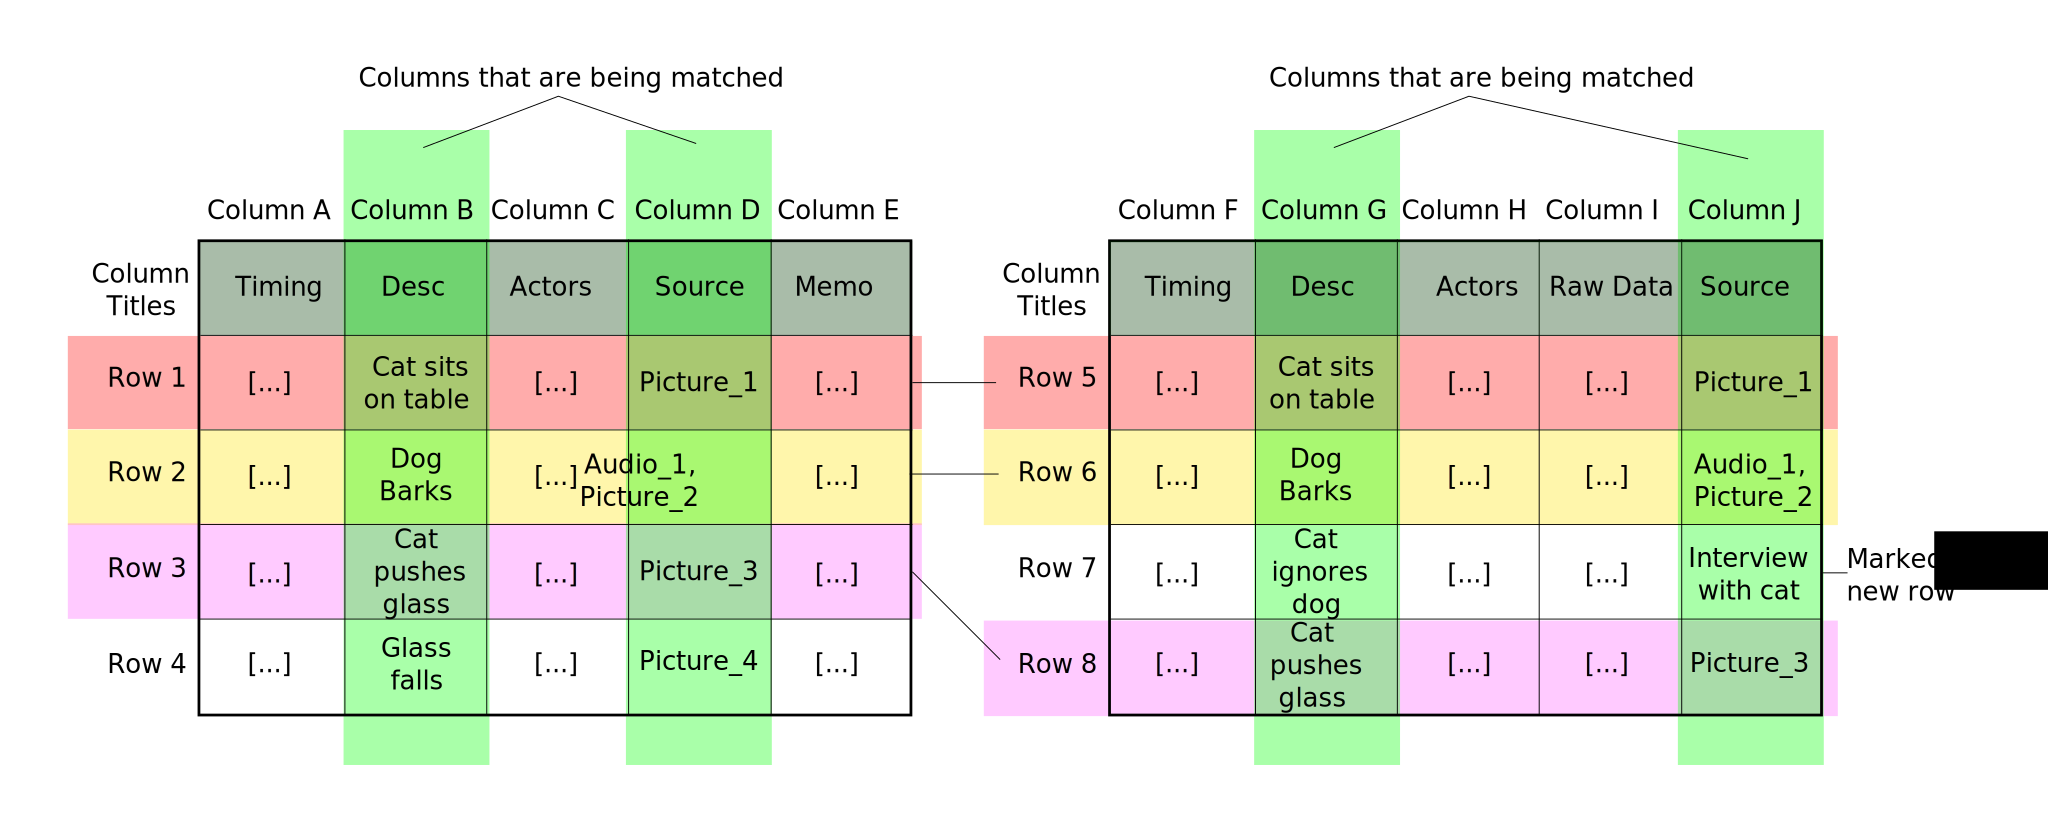
\includegraphics[width=100mm]{Diagram_1.pdf}
  \label{fig:importingcodesdiagram}
\end{figure}

\subsection{Problems when importing codes}
\label{sec:problemsimportingcodes}

There are several things that could go wrong when importing codes from an old data set into a new one. One problem would occur if you do not select any columns to be imported in the appropriate dialog. In this case the program will simply report that no columns were selected, and take no further action. Another similar problem would occur if you try to import codes from a data set that has now columns in common with the data set that is loaded into your current session. In this case the dialog where columns can be selected will be empty (except for the option to mark new entries). If you try to proceed, the program will behave as if no columns were selected (see above), report an error, and take no further action.

Another problem may be that some of the codes assigned to entries in the \textbf{old version} of the data set do not get imported into the \textbf{new version} of the data set, even though these entries appear in both. This should only happen if something changed in the contents of these entries (and only in the contents of those columns that the program tries to match). Even if you made only small changes in the contents of the selected columns, the program will treat the corresponding entry as a new, uncoded entry. 

A more difficult problem will occur if you do not select columns that allow the program to identify each row of data in the \textbf{old version} and/or the \textbf{new version} of your data set individually (see the box below for an explanation).

\begin{framed}
  \textbf{Example to illustrate problem when importing non-unique rows}

  First, imagine that you select two columns (\(C_1\) and \(C_2\)), the contents of which need to be matched by the program. Second, imagine that in the \textbf{old version} of the data set, there exist two incidents (two rows in the data set; \(I^{old}_1\) and \(I^{old}_2\)) that have identical data in those columns. In addition, imagine that the sets of codes (\(S_1\) and \(S_2\)) that you assigned to these two incidents are different (\(S_1 \rightarrow I^{old}_1\) and \(S_2 \rightarrow I^{old}_2\)).

  When comparing the two versions of the data set, the program encounters one of these rows of data \(I^{old}_1\). If it also encounters a row of data in the \textbf{new version} of the data set that has the exact same data in \(C_1\) and \(C_2\) (let us call this row \(I^{new}_x\)), it will think it has found a match, and assign the corresponding codes to the corresponding entry in the \textbf{new version} of the data set (\(S_1 \rightarrow I^{old}_1\) becomes \(S_1 \rightarrow I^{new}_x\)). However, the program then proceeds, and it will also encounter the other row of data \(I^{old}_2\), the contents of which (in columns \(C_1\) and \(C_2\)) also match with those of \(I^{new}_x\). As a result, the program will simply overwrite the codes that already existed (\(S_1 \rightarrow I^{new}_x\) gets overwritten by \(S_2 \rightarrow I^{new}_x\)). More importantly, the program will not recognise that something has gone wrong, so it will do this work silently, without reporting any error (also see figure \ref{fig:overwritingcodes}).
\end{framed}

\begin{figure}[h!]
  \centering
  \caption{Codes that are silently overwritten due to multiple matches.}
  \includegraphics[width=100mm]{Diagram_2.pdf}
  \label{fig:overwritingcodes}
\end{figure}

To prevent this problem from occurring, you must always make sure that, based on the columns that you selected in the import dialog, the program will never find two rows of data that are exactly the same. As explained in section \ref{sec:importingcodes}, it should typically be enough to select (1) a column that indicates the timing of the incident, and (2) a column that contains the qualitative description of the incident itself (see section \ref{sec:datasets} for the assumptions that the program makes about how your data set is structured). It is unlikely that two incidents have the exact same contents in these two columns (because then they would simply refer to the exact same incident).

\section{Navigating through the data}
\label{sec:navigatingdata}

The program, to some extent, enforces a specific way to walk through your data set. As explained in section \ref{sec:datasets}, the program assumes that your data are chronologically ordered, with the incidents that occurred earliest at the top, and the incidents that occurred latest at the bottom. When you start coding a new data set, the program will always assume that you wish to start the coding process with the earliest incident. The program will present to you one incident at a time, showing you details on the currently selected incident in up to two fields (see figure \ref{fig:incidentsoverview}). 

\begin{figure}[h!]
  \centering
  \caption{Overview of incident navigation section.}
  \includegraphics[width=100mm]{Screenshot_4.pdf}
  \label{fig:incidentsoverview}
\end{figure}

In the two fields, the program can display the contents of any of the columns of your original data set. Below each field, you will find buttons that you can use to choose which column of the original data set to display in the field (the first column of data is selected by default for both fields). The arrow buttons will go to the previous or next column, and the drop-down menu can be used to simply jump to a specific column. 

Typically, you will want to assign codes to the incidents based on the information provided in one or more columns of data, such as the description of the (inter)action that the incident captures, and possibly the raw text (from the sources of data) on which this description is based. The program can show up to two columns of data, which, in my own experience, is a nice balance between having a good overview, and not having to process too much information at a time.   

\subsection{Marking incidents}
\label{sec:markingincidents}



\chapter{Contact details}
\label{chap:contactdetails}





\end{document}